\documentclass[12pt]{article}

% Packages
\usepackage[margin=1in]{geometry}
\usepackage{amsmath,amssymb,amsthm}
\usepackage{enumitem}
\usepackage{hyperref}
\usepackage{xcolor}
\usepackage{import}
\usepackage{xifthen}
\usepackage{pdfpages}
\usepackage{transparent}
\usepackage{listings}
\usepackage{tikz}
\usepackage{physics}
\usepackage{siunitx}
\usepackage{booktabs}
\usepackage{cancel}
  \usetikzlibrary{calc,patterns,arrows.meta,decorations.markings}


\DeclareMathOperator{\Log}{Log}
\DeclareMathOperator{\Arg}{Arg}

\lstset{
    breaklines=true,         % Enable line wrapping
    breakatwhitespace=false, % Wrap lines even if there's no whitespace
    basicstyle=\ttfamily,    % Use monospaced font
    frame=single,            % Add a frame around the code
    columns=fullflexible,    % Better handling of variable-width fonts
}

\newcommand{\incfig}[1]{%
    \def\svgwidth{\columnwidth}
    \import{./Figures/}{#1.pdf_tex}
}
\theoremstyle{definition} % This style uses normal (non-italicized) text
\newtheorem{solution}{Solution}
\newtheorem{proposition}{Proposition}
\newtheorem{problem}{Problem}
\newtheorem{lemma}{Lemma}
\newtheorem{theorem}{Theorem}
\newtheorem{remark}{Remark}
\newtheorem{note}{Note}
\newtheorem{definition}{Definition}
\newtheorem{example}{Example}
\newtheorem{corollary}{Corollary}
\theoremstyle{plain} % Restore the default style for other theorem environments
%

% Theorem-like environments
% Title information
\title{Discretizing the Heat Equation in 2D}
\author{Jerich Lee}
\date{2024-12-11}

\begin{document}

\maketitle


\begin{solution}

    \begin{enumerate}
        \item \subsubsection*{Update Scheme for Interior Nodes}

        The explicit update scheme for interior nodes is derived from the PDE from the problem:
        \begin{align}
        \rho c \frac{\partial T}{\partial t} = k \left( \frac{\partial^2 T}{\partial x^2} + \frac{\partial^2 T}{\partial y^2} \right) + Q(x, y, t),
        \end{align}
        where $\rho$ is the density, $c$ is the heat capacity, $k$ is the thermal conductivity, $T$ is the temperature, and $Q$ is the heat source.
        
         We proceed by discretizing this equation in space and time. Consider a uniform spatial grid with spacing $\Delta x$ in the $x$-direction and $\Delta y$ in the $y$-direction, and a uniform time step $\Delta t$. We define:
        \begin{align}
        T_{i,j}^n \approx T(x_i, y_j, t_n),
        \end{align}
        where $x_i = i \Delta x$, $y_j = j \Delta y$, and $t_n = n \Delta t$.
        
         First, we approximate the time derivative $\frac{\partial T}{\partial t}$ using a forward difference:
        \begin{align}
        \frac{\partial T}{\partial t}(x_i, y_j, t_n) \approx \frac{T_{i,j}^{n+1} - T_{i,j}^n}{\Delta t}.
        \end{align}
        
         Next, we discretize the spatial second derivatives using central differences. For the $x$-direction:
        \begin{align}
        \frac{\partial^2 T}{\partial x^2}(x_i, y_j, t_n) \approx \frac{T_{i+1,j}^n - 2T_{i,j}^n + T_{i-1,j}^n}{\Delta x^2}.
        \end{align}
        
         Similarly, in the $y$-direction:
        \begin{align}
        \frac{\partial^2 T}{\partial y^2}(x_i, y_j, t_n) \approx \frac{T_{i,j+1}^n - 2T_{i,j}^n + T_{i,j-1}^n}{\Delta y^2}.
        \end{align}
        
         The source term $Q(x_i,y_j,t_n)$ is approximated as $Q_{i,j}^n$.
        
         Substituting these finite-difference approximations back into the PDE, we have:
        \begin{align}
        \rho c \frac{T_{i,j}^{n+1} - T_{i,j}^n}{\Delta t} = k \left( \frac{T_{i+1,j}^n - 2T_{i,j}^n + T_{i-1,j}^n}{\Delta x^2} + \frac{T_{i,j+1}^n - 2T_{i,j}^n + T_{i,j-1}^n}{\Delta y^2} \right) + Q_{i,j}^n.
        \end{align}
        
         Finally, we solve for $T_{i,j}^{n+1}$:
        \begin{align}
        T_{i,j}^{n+1} &= T_{i,j}^n + \frac{\Delta t}{\rho c}\bigg[ k\bigg( \frac{T_{i+1,j}^n - 2T_{i,j}^n + T_{i-1,j}^n}{\Delta x^2} + \frac{T_{i,j+1}^n - 2T_{i,j}^n + T_{i,j-1}^n}{\Delta y^2} \bigg) + Q_{i,j}^n \bigg]. \label{eqn7}
        \end{align}
        
         This is the explicit update formula for the interior nodes. Every new time step $T_{i,j}^{n+1}$ is computed explicitly using known values from the current time step $T_{i,j}^n$. The terms involving second derivatives handle heat diffusion, while the $Q_{i,j}^n$ term accounts for the heat source.

        \item \subsubsection*{Update Scheme for Boundary Nodes}

        For the left, right, and top boundaries, the heat loss is modeled by a non-linear radiation heat flux:
        \begin{align}
        k \frac{\partial T}{\partial n} = q_\text{rad},
        \end{align}
        where $q_\text{rad} = -\sigma \epsilon \left( T^4 - T_\infty^4 \right)$, and $T_\infty$ is the ambient temperature. The normal derivative $\frac{\partial T}{\partial n}$ is approximated using first-order one-sided differences.
        
        \subsubsection*{Discretization of Boundary Conditions}
        
        1. Left Boundary ($i=0$):  
           The temperature gradient at the left boundary is approximated as:
           \begin{align}
           \frac{\partial T}{\partial x} \bigg|_{x=0} \approx \frac{T_{1,j}^n - T_{0,j}^n}{\Delta x}.
           \end{align}
           Substituting into the boundary condition:
           \begin{align}
           k \frac{T_{1,j}^n - T_{0,j}^n}{\Delta x} = -\sigma \epsilon \left( (T_{0,j}^n)^4 - T_\infty^4 \right).
           \end{align}
           Rearranging gives a non-linear equation for $T_{0,j}^n$:
           \begin{align}
           T_{0,j}^n = T_{1,j}^n - \frac{\Delta x \, \sigma \epsilon}{k} \left( (T_{0,j}^n)^4 - T_\infty^4 \right).
           \end{align}
           This equation is solved iteratively using Newton's method.
        
        2. Right Boundary ($i=N_x$):  
           Similarly, the right boundary condition is:
           \begin{align}
           \frac{\partial T}{\partial x} \bigg|_{x=L_x} \approx \frac{T_{N_x,j}^n - T_{N_x-1,j}^n}{\Delta x}.
           \end{align}
           Substituting into the boundary condition:
           \begin{align}
           k \frac{T_{N_x,j}^n - T_{N_x-1,j}^n}{\Delta x} = -\sigma \epsilon \left( (T_{N_x,j}^n)^4 - T_\infty^4 \right).
           \end{align}
           Solving for $T_{N_x,j}^n$ follows the same iterative approach.
        
        3. Top Boundary ($j=N_y$):  
           For the top boundary:
           \begin{align}
           \frac{\partial T}{\partial y} \bigg|_{y=L_y} \approx \frac{T_{i,N_y}^n - T_{i,N_y-1}^n}{\Delta y}.
           \end{align}
           Substituting into the boundary condition:
           \begin{align}
           k \frac{T_{i,N_y}^n - T_{i,N_y-1}^n}{\Delta y} = -\sigma \epsilon \left( (T_{i,N_y}^n)^4 - T_\infty^4 \right).
           \end{align}
        
        \subsubsection*{Numerical Solution for Non-Linear Boundary Conditions}
        
        We will handle the non-linear equation for each boundary node by solving them iteratively using Newton-Raphson:
        \begin{align}
        f(T_\text{bnd}) = k \frac{T_\text{bnd} - T_\text{inboard}}{\Delta} + \sigma \epsilon \left( T_\text{bnd}^4 - T_\infty^4 \right)\label{eqn16}, 
        \end{align}
        where $T_\text{bnd}$ is the boundary temperature, $T_\text{inboard}$ is the adjacent interior temperature, and $\Delta$ is the grid spacing. The derivative for Newton's method is:
        \begin{align}
        f'(T_\text{bnd}) = \frac{k}{\Delta} + 4 \sigma \epsilon T_\text{bnd}^3.
        \end{align}
        
        At each time step, for each boundary node:
    \begin{enumerate}
        \item 
        1. The previous time step's $T_\text{bnd}$ will be used as an initial guess.
    \item 
        2. We will iteratively solve $f(T_\text{bnd}) = 0$ until convergence.
    \end{enumerate}
        
        
    The interior temperatures are used to approximate gradients, and Newton-Raphson ensures convergence of the boundary temperatures.
    \end{enumerate}
\end{solution}

\begin{solution}
    

        For Question 2, we will implement a stationary laser source at the midpoint of the top domain and select time step $\Delta t = 0.01$ seconds.


            \subsubsection*{Problem Parameters:}  
            We have a stationary laser located at $ x_L = 0.5L_x, y = L_y $. Parameters from Table 2 are:
            \begin{align}
            P = 800\ \text{W}, \quad N_x = 50, \quad N_y = 50, \quad t_\text{end} = 150\ \text{s}.
            \end{align}
            We will model the 2D transient heat equation:
            \begin{align}
            \rho c \frac{\partial T}{\partial t} = k\left( \frac{\partial^2 T}{\partial x^2} + \frac{\partial^2 T}{\partial y^2} \right) + Q(x,y,t),
            \end{align}
            with the laser source term $ Q(x,y,t) $ given by:
            \begin{align}
            Q(x,y,t) = \left(\frac{P}{w^2 \sqrt{2\pi}}\right)\exp\left(-\frac{(x - x_L)^2}{2w^2}\right)f(y),
            \end{align}
            where
            \begin{align}
            f(y) = \frac{\beta}{L_y}\exp\left(-\beta\frac{L_y - y}{L_y}\right).
            \end{align}
        
            Since the laser is stationary, $ x_L $ is constant in time.
        
            \subsubsection*{Discretization:}  
            With $ N_x = 50 $ and $ N_y = 50 $, we have:
            \begin{align}
            \Delta x = \frac{L_x}{N_x}, \quad \Delta y = \frac{L_y}{N_y}.
            \end{align}
            Time is discretized with $\Delta t$. The explicit scheme is given by \autoref{eqn7} and shown below:
            \begin{align}
            T_{i,j}^{n+1} = T_{i,j}^n + \frac{\Delta t}{\rho c}\left[ k\left(\frac{T_{i+1,j}^n - 2T_{i,j}^n + T_{i-1,j}^n}{\Delta x^2} + \frac{T_{i,j+1}^n - 2T_{i,j}^n + T_{i,j-1}^n}{\Delta y^2}\right) + Q_{i,j}^n \right].
            \end{align}
        
            \subsubsection*{Boundary Conditions:}  
            \begin{enumerate}
            \item Bottom ($y=0$): Fixed at $\tilde{T}=298\ \text{K}$.  
            \item Left, Right, and Top: Radiation boundary conditions as before, solved using a non-linear approach in \autoref{eqn16}.
            \end{enumerate}
        
            \subsubsection*{Stability Analysis}  
             To derive the stability constraint for the explicit finite-difference scheme, we will use von Neumann stability analysis. Starting from the discrete update scheme for the 2D heat equation (\autoref{eqn7}), we focus on the homogeneous form (no source term $Q$):
\begin{align}
T_{i,j}^{n+1} = T_{i,j}^n + \frac{\Delta t}{\rho c}\left[ k \left( \frac{T_{i+1,j}^n - 2T_{i,j}^n + T_{i-1,j}^n}{\Delta x^2} + \frac{T_{i,j+1}^n - 2T_{i,j}^n + T_{i,j-1}^n}{\Delta y^2}\right) \right].
\end{align}

 For the stability analysis, we assume a solution of the form:
\begin{align}
T_{i,j}^n = \lambda^n e^{i(\alpha i + \beta j)},
\end{align}
where $\alpha$ and $\beta$ are wave numbers in the $x$ and $y$ directions, respectively, and $\lambda$ is the amplification factor per time step. We substitute this trial solution into the homogeneous version of the update equation and look for conditions on $\Delta t$ that ensure $|\lambda| \leq 1$ for stability.

 Substitute $T_{i,j}^n = \lambda^n e^{i(\alpha i + \beta j)}$ into the discrete Laplacian terms:
\begin{align}
T_{i+1,j}^n &= \lambda^n e^{i[\alpha(i+1) + \beta j]} = \lambda^n e^{i\alpha}e^{i(\alpha i + \beta j)}, \\
T_{i-1,j}^n &= \lambda^n e^{i[\alpha(i-1) + \beta j]} = \lambda^n e^{-i\alpha}e^{i(\alpha i + \beta j)}, \\
T_{i,j+1}^n &= \lambda^n e^{i[\alpha i + \beta (j+1)]} = \lambda^n e^{i\beta}e^{i(\alpha i + \beta j)}, \\
T_{i,j-1}^n &= \lambda^n e^{i[\alpha i + \beta (j-1)]} = \lambda^n e^{-i\beta}e^{i(\alpha i + \beta j)}.
\end{align}

 Factor out $\lambda^n e^{i(\alpha i + \beta j)}$:
\begin{align}
\frac{T_{i+1,j}^n - 2T_{i,j}^n + T_{i-1,j}^n}{\Delta x^2} &= \frac{\lambda^n e^{i(\alpha i + \beta j)}}{\Delta x^2} (e^{i\alpha} - 2 + e^{-i\alpha}), \\
\frac{T_{i,j+1}^n - 2T_{i,j}^n + T_{i,j-1}^n}{\Delta y^2} &= \frac{\lambda^n e^{i(\alpha i + \beta j)}}{\Delta y^2} (e^{i\beta} - 2 + e^{-i\beta}).
\end{align}

 Note that $(e^{i\theta} - 2 + e^{-i\theta}) = -2 + (e^{i\theta} + e^{-i\theta}) = -2 + 2\cos\theta = 2(\cos\theta - 1)$.

 Thus:
\begin{align}
\frac{T_{i+1,j}^n - 2T_{i,j}^n + T_{i-1,j}^n}{\Delta x^2} = \frac{\lambda^n e^{i(\alpha i + \beta j)}}{\Delta x^2} \cdot 2(\cos\alpha - 1),
\end{align}
\begin{align}
\frac{T_{i,j+1}^n - 2T_{i,j}^n + T_{i,j-1}^n}{\Delta y^2} = \frac{\lambda^n e^{i(\alpha i + \beta j)}}{\Delta y^2} \cdot 2(\cos\beta - 1).
\end{align}

 The update equation becomes:
\begin{align}
\lambda^{n+1} e^{i(\alpha i + \beta j)} = \lambda^n e^{i(\alpha i + \beta j)} + \frac{\Delta t}{\rho c} \left[ k \left( \frac{2(\cos\alpha - 1)}{\Delta x^2} + \frac{2(\cos\beta - 1)}{\Delta y^2} \right)\lambda^n e^{i(\alpha i + \beta j)} \right].
\end{align}

 Canceling $\lambda^n e^{i(\alpha i + \beta j)}$:
\begin{align}
\lambda = 1 + \frac{\Delta t k}{\rho c}\left( \frac{2(\cos\alpha - 1)}{\Delta x^2} + \frac{2(\cos\beta - 1)}{\Delta y^2}\right).
\end{align}

 Since $|\cos\theta - 1| \leq 0$, the most restrictive case occurs when $\cos\alpha = \cos\beta = -1$, which gives the largest magnitude of negative shift, i.e. $\cos\theta - 1 = -2$. Substituting $\cos\alpha = \cos\beta = -1$:
\begin{align}
\lambda = 1 + \frac{\Delta t k}{\rho c}\left(\frac{2(-2)}{\Delta x^2} + \frac{2(-2)}{\Delta y^2}\right) = 1 - \frac{4\Delta t k}{\rho c}\left( \frac{1}{\Delta x^2} + \frac{1}{\Delta y^2}\right).
\end{align}

 For stability, we require $|\lambda| \leq 1$. The most important condition is $\lambda \geq -1$, as $\lambda \leq 1$ is implied if $\lambda < 1$. Thus:
\begin{align}
-1 \leq 1 - \frac{4\Delta t k}{\rho c}\left( \frac{1}{\Delta x^2} + \frac{1}{\Delta y^2} \right).
\end{align}

 Solve for $\Delta t$:
\begin{align}
-1 \leq 1 - \frac{4\Delta t k}{\rho c}\left( \frac{1}{\Delta x^2} + \frac{1}{\Delta y^2} \right) &\implies -2 \leq - \frac{4\Delta t k}{\rho c}\left( \frac{1}{\Delta x^2} + \frac{1}{\Delta y^2}\right) \\
\implies \frac{4 \Delta t k}{\rho c}\left( \frac{1}{\Delta x^2} + \frac{1}{\Delta y^2}\right) \leq 2 \\
\implies \Delta t \leq \frac{\rho c}{2k}\left(\frac{1}{\Delta x^2} + \frac{1}{\Delta y^2}\right)^{-1}.
\end{align}

 This is the stability constraint that ensures the explicit scheme remains stable. It shows that the time step must be small enough relative to the spatial discretization and material properties.
            \begin{align}
            r_x = \frac{k \Delta t}{\rho c \Delta x^2}, \quad r_y = \frac{k \Delta t}{\rho c \Delta y^2}, \quad \text{and we require } r_x + r_y < 0.5.
            \end{align}
        
             We have chosen $\Delta t = 0.01$ seconds. To verify that a time step of $\Delta t = 0.01\,\text{s}$ satisfies the stability constraint, we begin with the derived inequality:
            \begin{align}
            \Delta t \leq \frac{\rho c}{2k} \left( \frac{1}{\Delta x^2} + \frac{1}{\Delta y^2} \right)^{-1}.
            \end{align}
            
             We know the physical and numerical parameters: $\rho$, $c$, $k$, $\Delta x$, and $\Delta y$. We proceed by computing the allowable maximum $\Delta t_{\max}$.
            
            First, define:
            \begin{align}
            S = \frac{1}{\Delta x^2} + \frac{1}{\Delta y^2}.
            \end{align}
            Then:
            \begin{align}
            \Delta t_{\max} = \frac{\rho c}{2k}\cdot \frac{1}{S}.
            \end{align}
            
             Using the given problem parameters:
            \begin{align}
            \rho = 7900\,\text{kg/m}^3, \quad c = 470\,\text{J/(kg·K)}, \quad k = 48\,\text{W/(m·K)},
            \end{align}
            assuming:
            \begin{align}
            \Delta x = \Delta y = 0.001\,\text{m},
            \end{align}
            then:
            \begin{align}
            \frac{1}{\Delta x^2} = \frac{1}{(0.001)^2} = 10^6.
            \end{align}
            Since $\Delta x = \Delta y$, we have:
            \begin{align}
            S = 10^6 + 10^6 = 2 \times 10^6.
            \end{align}
            
             Next, we compute $\frac{\rho c}{2k}$:
            \begin{align}
            \rho c = 7900 \times 470 = 3{,}713{,}000.
            \end{align}
            \begin{align}
            \frac{\rho c}{2k} = \frac{3{,}713{,}000}{2 \times 48} = \frac{3{,}713{,}000}{96} \approx 38{,}677.08.
            \end{align}
            
             Therefore:
            \begin{align}
            \Delta t_{\max} = 38{,}677.08 \cdot \frac{1}{2 \times 10^6} = 38{,}677.08 \times 5 \times 10^{-7} \approx 0.01934\,\text{s}.
            \end{align}
            
             As we have chosen $\Delta t = 0.01\,\text{s}$, we compare:
            \begin{align}
            0.01\,\text{s} \leq 0.01934\,\text{s}.
            \end{align}
            
             This inequality is true, so $\Delta t = 0.01\,\text{s}$ is within the stability limit. Therefore, a time step of 0.01 seconds works for the given parameters and ensures the numerical stability of the explicit scheme.
        
        
        \begin{enumerate}
            

        \item Table for Question 2.1: \begin{table}[h!]
            \centering
            \begin{tabular}{|c|c|}
                \hline
                Time (s) & Max Temperature at Top Surface (K) \\ \hline
                30.00 & 1661.53 \\ \hline
                60.00 & 1880.57 \\ \hline
                90.00 & 1932.01 \\ \hline
                120.00 & 1943.73 \\ \hline
                150.00 & 1946.39 \\ \hline
            \end{tabular}
            \caption{Maximum temperature at the top surface of the domain at selected times.}
            \label{tab:maxtemp}
        \end{table}
    \item The plots of temperature vs time at $x = 0.5L_x$ at the top surface ($y = L_y$), 20\% depth ($y = 0.8L_y$), and 50\% depth ($y = 0.5L_y$) are shown in \autoref{fig:1}
     \begin{figure}[htbp]
        \centering
        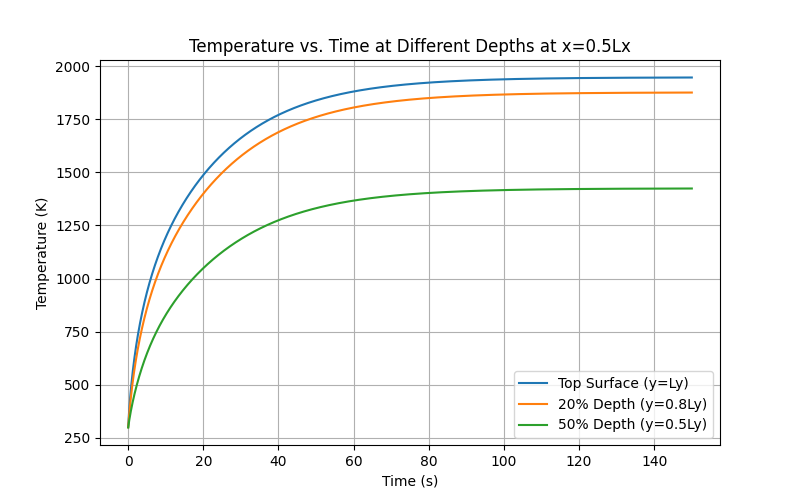
\includegraphics[width=0.8\textwidth]{classes/fall-2024/tam-470/diary/12-09/Figure_2-proj2.png}
        \caption{Temperature vs Time at Different Depths}
        \label{fig:1}
    \end{figure}
    \item A plot of temperature vs position at the final time along the line $x = 0.5L_x$ is shown in \autoref{fig:2}
     \begin{figure}[htbp]
        \centering
        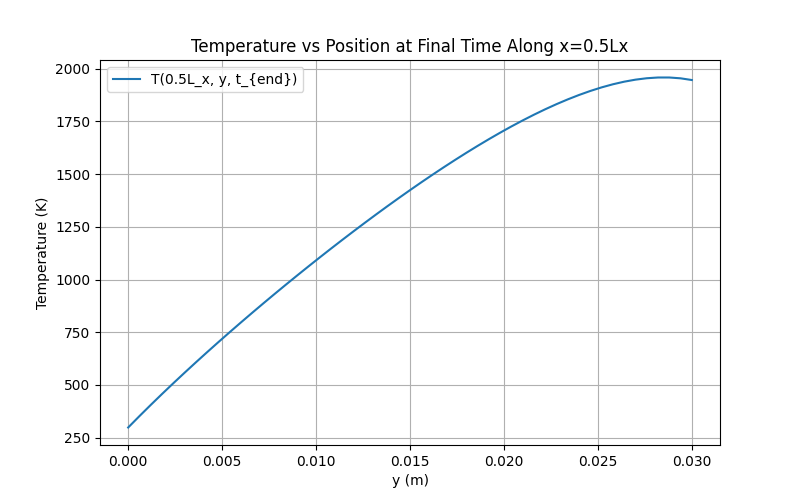
\includegraphics[width=0.8\textwidth]{classes/fall-2024/tam-470/diary/12-09/Figure_3-proj-2.png}
        \caption{Temperature vs position at the final time along the line $x = 0.5L_x$}
        \label{fig:2}
    \end{figure}
    \item Contour plots of temperature distribution throughout the domain at t = 10, 40, 150
    second:
    \begin{enumerate}
        \item \autoref{fig:3} : \begin{figure}[htbp]

            \centering
            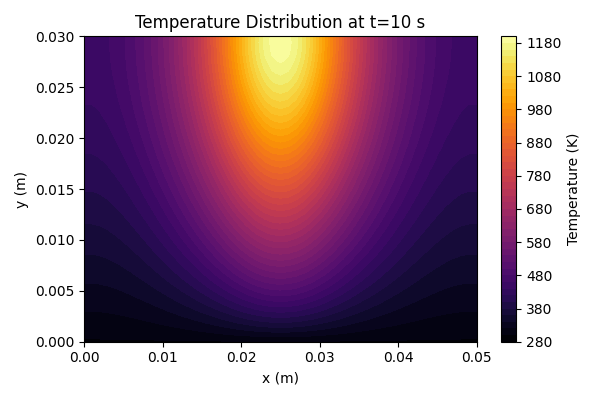
\includegraphics[width=0.8\textwidth]{classes/fall-2024/tam-470/diary/12-09/proj-2.2.4.1.png}
            \caption{t=10s}
            \label{fig:3}
        \end{figure}
        \item \autoref{fig:4}: \begin{figure}[htbp]
            \centering
            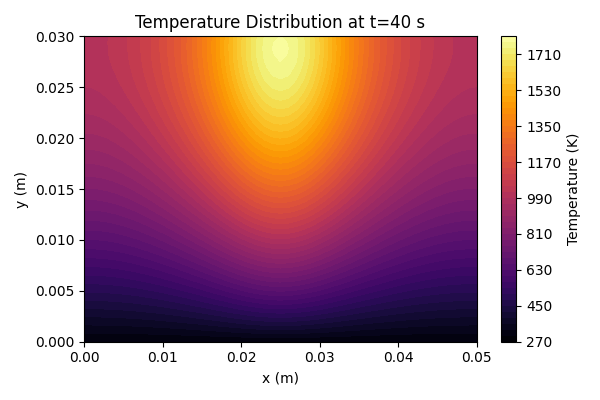
\includegraphics[width=0.8\textwidth]{classes/fall-2024/tam-470/diary/12-09/proj-2.2.4.2.png}
            \caption{t=40s}
            \label{fig:4}
        \end{figure}
    \item \autoref{fig:5}: \begin{figure}[htbp]
        \centering
        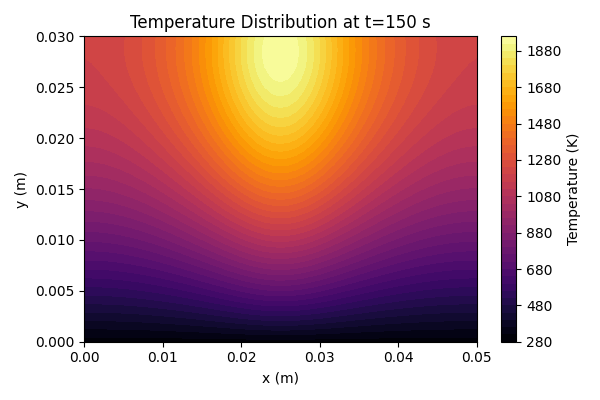
\includegraphics[width=0.8\textwidth]{classes/fall-2024/tam-470/diary/12-09/proj-2.2.4.3.png}
        \caption{t=40s}
        \label{fig:5}
    \end{figure}
    \end{enumerate}
    \item All of the plots look consistent with the input parameters of the given traversing laser heating system. The simulation plot shown in \autoref{fig:1} shows the overlain graphs of three depths, namely at $y=Ly, y=0.8L$ and $y=0.5Ly$. The values of the plots as the depth gets deeper results in a lower average temperature value, which is expected, as the volume closest to the top of the surface reach a higher temperature, and approaches a limiting point as time increasing—a trend consistent throughout each measured depth. In \autoref{fig:2}, the plot of the temperature vs. the position at the final time, $t=150$ seconds, is shown. The dominant trend is such that the graph is linear, with the exception of the tail, which has a slight curvature with decreasing behavior as the depth is increased, which matches the behavior exhibited in \autoref{fig:1}. The plots shown in \autoref{fig:3}, \autoref{fig:4}, and \autoref{fig:5}, which show the temperature distribution at time $t=10, 40, 150$ seconds display a temperature field with the highest temperatures forming closed to the laser's location and decaying as the spatial coordinates are increased from the laser source. These plots match the behavior of the previous figures.  
    \end{enumerate}

\end{solution}

\begin{solution}


When we use the same time step as in the previous question, $\Delta t=0.01$ seconds, the code terminates and converges.
     \begin{enumerate}
        \item \autoref{fig:6} \begin{figure}[htbp]
            \centering
            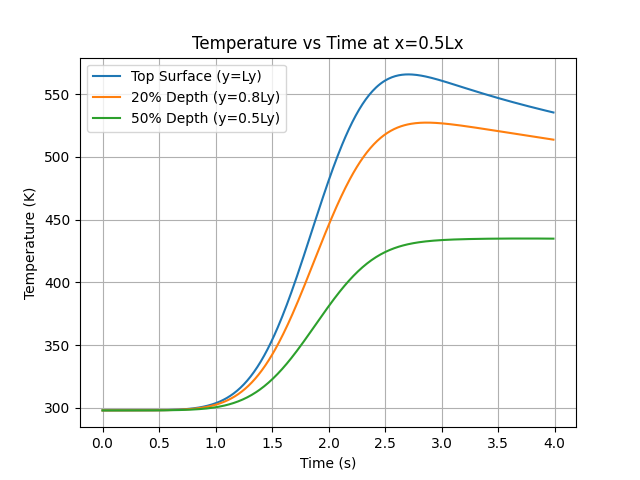
\includegraphics[width=0.8\textwidth]{classes/fall-2024/tam-470/diary/12-09/proj-2.3.1.png}
            \caption{Plots of temperature vs time at $x = 0.5L_x$ at the top surface ($y = L_y$), 20\% depth ($y = 0.8L_y$), and 50\% depth ($y = 0.5L_y$).}
            \label{fig:6}
        \end{figure}
        \item \begin{enumerate}
           \item  \autoref{fig:7} \begin{figure}[htbp]
            \centering
            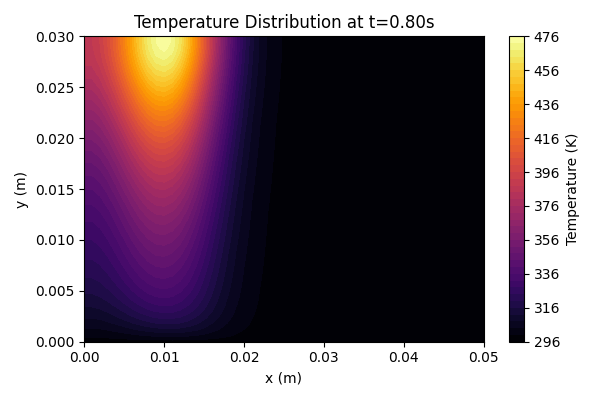
\includegraphics[width=0.8\textwidth]{classes/fall-2024/tam-470/diary/12-09/proj-2.3.2.png}
            \caption{Contour plots of temperature distribution in the domain at $t = 0.2t_\text{end}$ seconds}
            \label{fig:7}
        \end{figure}
        \item \autoref{fig:8} \begin{figure}[htbp]
            \centering
            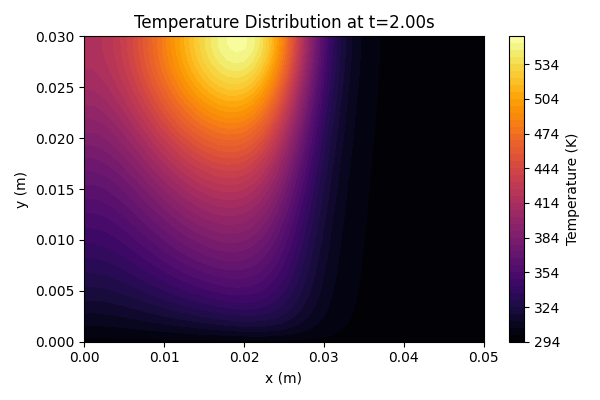
\includegraphics[width=0.8\textwidth]{classes/fall-2024/tam-470/diary/12-09/proj-2.3.3.png}
            \caption{Contour plots of temperature distribution in the domain at $t = 0.5t_\text{end}$ seconds}
            \label{fig:8}
        \end{figure}
    \item \autoref{fig:9} \begin{figure}[htbp]
        \centering
        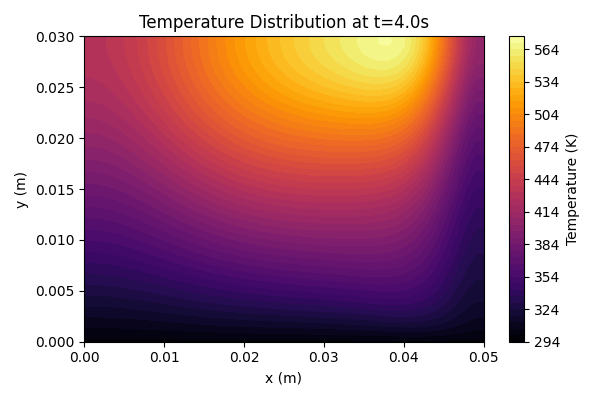
\includegraphics[width=0.8\textwidth]{classes/fall-2024/tam-470/diary/12-09/proj-2.3.4.png}
        \caption{Contour plots of temperature distribution in the domain at $t = t_\text{end}$ seconds}
        \label{fig:9}
    \end{figure}
        \end{enumerate}
        \item The simulation results show that the as the laser traverses across the surface of the given domain, the temperature field responds in a manner that makes sense with the given problem and is consistent with the expected physical behavior. Taking a look at \autoref{fig:7}, \autoref{fig:8}, and \autoref{fig:9}, we see that the temperature increases as the $x$ value of the domain is increased, i.e., as the laser travels from left to right. This matches \autoref{fig:6}, as this is a plot that measures the temperature distribution as a single point, namely at the midpoint of the $x$ domain. This plot corresponds to the temperature distribution plots, as \autoref{fig:6} shows a logistic type curve, with small values at early time values, then increasing rapidly, followed by a slow decreasing tail approaching a limit point. This matches the temperature plots because at the midpoint of the domain, the domain should not experience any heat, as the laser starts at the very left of the domain. 
        \end{enumerate}

\end{solution}

\begin{solution}
    
    \begin{enumerate}
        \item \autoref{fig:10} \begin{figure}[htbp]
            \centering
            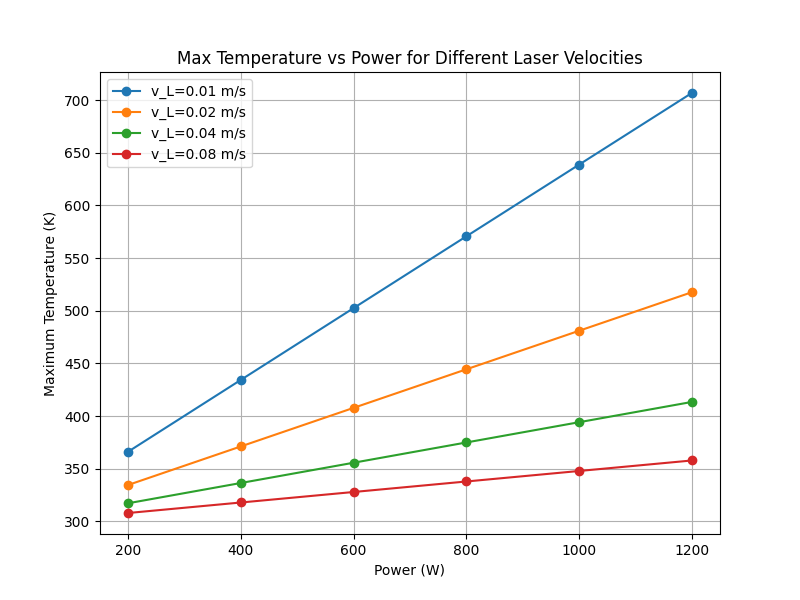
\includegraphics[width=0.8\textwidth]{classes/fall-2024/tam-470/diary/12-09/proj-2.4.1.png}
            \caption{Maximum temperature on the vertical axis vs power}
            \label{fig:10}
        \end{figure}
    \item The plot in \autoref{fig:10} shows the maximum temperature vs. power for different laser velocities. The most obvious trend is that as the velocity of the laser decreased, the rate of the maximum temperature for each laser velocity increased; i.e., the behavior of each velocity when plotted for power vs temperature showed increasing, linear behavior. Intuitively, this demonstrates that as the rate of the movement of the laser decreases, the domain of the system has more time to heat, allowing for an accumulated heat build up, resulting in a larger maximum temperature. 
    At higher speeds, the laser has less time to concentrate its energy on a point and its neighbors, which leads to distributing heat more superficially, which leads to a lower linear slope value. 
    \end{enumerate}
\end{solution}
\end{document}
